%%%%%%%%%%%%%%%%%%%%%%%%%%%%%%%%%%%%%%%%%%%%%%%%%%%%%%%%%%%%%%%%
%%                                                            %%
%% aGreekPrimer, Italian translation 2016.12 - 2017           %%
%%                                                            %%
%% From:  Clarence W. Gleason, A Greek Primer                 %%
%%        (1903, New York, American Book Company)             %%
%%                                                            %%
%%        https://archive.org/details/greekprimer00glea       %%
%%                                                            %%
%% Translated by g.p.ciceri <gp.ciceri@gmail.com>             %%
%% ---------------------------------------------------------- %%
%% This translation is Licensed under                         %%
%% Creative Commons Attribution-ShareAlike 4.0 International  %%
%% https://creativecommons.org/licenses/by-sa/4.0/            %%
%%                                                            %%
%%%%%%%%%%%%%%%%%%%%%%%%%%%%%%%%%%%%%%%%%%%%%%%%%%%%%%%%%%%%%%%%

% ᾶῖῶῆῦ  
% ἀἰὐἐὀὠἠ 
% ὰὲὶὸὺὼὴ 
% ἁἱὑὁὡἡῥ
% άέίόύήώΆΉ
% ἂἒὒἲὂὢἢὒἚἊ
% ἃἳὓὃἣὣἓἋἛ
% ἄἔἴὄὔὤἤἌἬ
% ἅἕἵὅὕὥἥἍἭ
% ἆὦἶἦὖἯἏὯἇὧἷἧὗἯἏὯ 

% ᾳῃῳ
% ᾱῑῡ
% ᾀᾐᾠ
% ᾰῐῠ
% ᾂᾒᾢ
% ϊ ϋ
% ᾄᾔᾤ
% ΰ ΐ
% ᾆᾖᾦ
% ᾲῂῲ
% ᾴῄῴ
% ᾷῇῷ


\documentclass[nols]{tufte-handout}

%\geometry{showframe} % display margins for debugging page layout

\usepackage{fontspec}
\usepackage{ifxetex}
\setmainfont[Path=./fonts/palatino-linotype/, ItalicFont=palai.ttf, BoldFont=palab.ttf]{pala.ttf}
%\setmainfont[Path=./fonts/GFS_Didot/, ItalicFont=GFSDidotItalic.ttf, BoldFont=GFSDidotBold.ttf]{GFSDidot.ttf}

\newfontfamily\GFSDidotBf[Path=./fonts/GFS_Didot/]{GFSDidotBold.ttf}
\newfontfamily\GFSDidot[Path=./fonts/GFS_Didot/]{GFSDidot.ttf}

\newcommand{\didobf}[1]{{\GFSDidotBf #1}}
\newcommand{\dido}[1]{{\GFSDidot #1}}

\usepackage{lipsum}
\usepackage{url}
\usepackage{longtable}
\usepackage{stackengine}

\usepackage{graphicx} % allow embedded images
  \setkeys{Gin}{width=\linewidth,totalheight=\textheight,keepaspectratio}
  \graphicspath{{graphics/}} % set of paths to search for images
\usepackage{amsmath}  % extended mathematics
\usepackage{booktabs} % book-quality tables
\usepackage{units}    % non-stacked fractions and better unit spacing
\usepackage{multicol} % multiple column layout facilities
\usepackage{lipsum}   % filler text
\usepackage{fancyvrb} % extended verbatim environments
  \fvset{fontsize=\normalsize}% default font size for fancy-verbatim environments

% Standardize command font styles and environments
\newcommand{\doccmd}[1]{\texttt{\textbackslash#1}}% command name -- adds backslash automatically
\newcommand{\docopt}[1]{\ensuremath{\langle}\textrm{\textit{#1}}\ensuremath{\rangle}}% optional command argument
\newcommand{\docarg}[1]{\textrm{\textit{#1}}}% (required) command argument
\newcommand{\docenv}[1]{\textsf{#1}}% environment name
\newcommand{\docpkg}[1]{\texttt{#1}}% package name
\newcommand{\doccls}[1]{\texttt{#1}}% document class name
\newcommand{\docclsopt}[1]{\texttt{#1}}% document class option name
\newenvironment{docspec}{\begin{quote}\noindent}{\end{quote}}% command specification environment

% concetti morfosintattici
\usepackage{xspace} 
\newcommand{\noun}{\textsc{sostantivo}\xspace}
\newcommand{\nouns}{\textsc{sostantivi}\xspace}
\newcommand{\adject}{\textsc{aggettivo}\xspace}
\newcommand{\adjects}{\textsc{aggettivi}\xspace}
\newcommand{\gnumber}{\textsc{numero}\xspace}
\newcommand{\gnumbers}{\textsc{numeri}\xspace}
\newcommand{\gender}{\textsc{genere}\xspace}
\newcommand{\genders}{\textsc{generi}\xspace}
\newcommand{\gcase}{\textsc{caso}\xspace}
\newcommand{\gcases}{\textsc{casi}\xspace}
\newcommand{\tense}{\textsc{tempo}\xspace}
\newcommand{\mood}{\textsc{modo}\xspace}
\newcommand{\gverb}{\textsc{verbo}\xspace}
\newcommand{\gverbs}{\textsc{verbi}\xspace}
\newcommand{\adjective}{\textsc{aggettivo}\xspace}
\newcommand{\nom}{\textsc{nom}\xspace}
\newcommand{\gen}{\textsc{gen}\xspace}
\newcommand{\dat}{\textsc{dat}\xspace}
\newcommand{\acc}{\textsc{acc}\xspace}
\newcommand{\voc}{\textsc{voc}\xspace}
\newcommand{\gexit}{\textsc{uscita}\xspace}
\newcommand{\gexits}{\textsc{uscite}\xspace}
\newcommand{\declinazione}{\textsc{declinazione}\xspace}
\newcommand{\masc}{\textsc{maschile}\xspace}
\newcommand{\femm}{\textsc{femminile}\xspace}
\newcommand{\neut}{\textsc{neutro}\xspace}

\newcommand{\indic}{\textsc{indicativo}\xspace}
\newcommand{\imper}{\textsc{imperativo}\xspace}
\newcommand{\gcong}{\textsc{congiuntivo}\xspace}
\newcommand{\ott}{\textsc{ottativo}\xspace}
\newcommand{\partic}{\textsc{participio}\xspace}
\newcommand{\infin}{\textsc{infinito}\xspace}

\newcommand{\pres}{\textsc{presente}\xspace}
\newcommand{\imperf}{\textsc{imperfetto}\xspace}
\newcommand{\aor}{\textsc{aoristo}\xspace}
\newcommand{\fut}{\textsc{futuro}\xspace}

\newcommand{\sing}{\textsc{singolare}\xspace}
\newcommand{\plur}{\textsc{plurale}\xspace}
\newcommand{\dual}{\textsc{duale}\xspace}


% italianitudini
\renewcommand{\figurename}{Figura}
\renewcommand{\tablename}{Tabella}
\renewcommand{\contentsname}{Indice}

% fix per un qualche problema
\ifxetex
  \newcommand{\textls}[2][5]{%
    \begingroup\addfontfeatures{LetterSpace=#1}#2\endgroup
  }
  \renewcommand{\allcapsspacing}[1]{\textls[15]{#1}}
  \renewcommand{\smallcapsspacing}[1]{\textls[10]{#1}}
  \renewcommand{\allcaps}[1]{\textls[15]{\MakeTextUppercase{#1}}}
  \renewcommand{\smallcaps}[1]{\smallcapsspacing{\scshape\MakeTextLowercase{#1}}}
  \renewcommand{\textsc}[1]{\smallcapsspacing{\textsmallcaps{#1}}}
\fi

\title{A Greek Primer. Introduzione al Greco Antico \newline Lezione V - L'imperfetto indicativo attivo. L'aumento.}

\author[gpciceri]{a cura di Milagathòs: Milo's help to enjoy humanities}

\date{31 Dicembre 2016} % without \date command, current date is supplied


\begin{document}

\maketitle% this prints the handout title, author, and date

\begin{marginfigure}[-2.5cm]
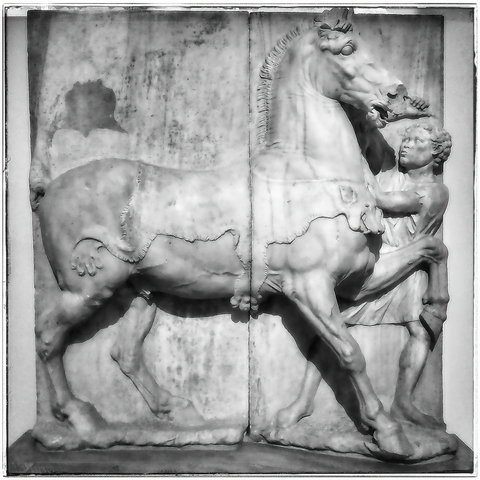
\includegraphics{smallthumb-lesson_I.jpeg}
\setfloatalignment{b}
\end{marginfigure}


\begin{abstract}
\noindent
Queste lezioni si articolano in \textsc{elementi grammaticali}, 
espressi sommariamente, seguiti da \textsc{vocabolari} per il lessico di base 
e da \textsc{frasi da tradurre} dal greco e in greco. 
\
L'approccio è quello del testo-laboratorio di morfosintassi: 
si presenta punto per punto - riprendendone la numerazione - 
l'esposizione di Gleason\cite{gleason1903}.\\
\bigskip
\noindent
Lezione V: l'imperfetto indicativo attivo, l'aumento sillabico e l'aumento temporale, le desinenze personali dei tempi secondari, vocabolario, esercizi.
\end{abstract}

%\printclassoptions

\newthought{73.} Nei tempi secondari\sidenote{imperfetto, aoristo, piuccheperfetto} dell'indicativo il verbo riceve, al suo inizio, un \textit{aumento}, che denota l'azione passata. 
L'aumento può essere di due tipi.

\newthought{74. Aumento sillabico} L'imperfetto e l'aoristo indicativo dei verbi che iniziano per consonante 
presentano come prefisso una sillaba \didobf{ε}, come in \didobf{ἔ-λυον} (imperfetto indicativo di \didobf{λύω}), \textit{io scioglievo}. 
Questo fenomeno viene detto \textit{aumento sillabico}.

\newthought{74. Aumento temporale} L'imperfetto e l'aoristo indicativo dei verbi che iniziano per vocale o per dittongo 
allungano la prima vocale, come in \didobf{ἦ-γον} (imperfetto indicativo di \didobf{ἄγω}), \textit{io conducevo}. 
\begin{multicols}{2}
    \noindent \hangindent=1em \didobf{α, ε} diventano \didobf{η}.  \\
	\noindent \hangindent=1em \didobf{ι, ο, υ} diventano \didobf{ῑ, ω, ῡ}.  \\
	\noindent \hangindent=1em \didobf{αι , ᾳ} diventano \didobf{ῃ}.  \\
	\noindent \hangindent=1em \didobf{οι} diventa \didobf{ῳ}.  \\
\end{multicols}
Questo fenomeno viene detto \textit{aumento temporale}.

\newthought{76. L'Imperfetto Indicativo Attivo}

\begin{fullwidth}
\begin{table}[!htbp]
  \centering
  \begin{tabular}{l l l l l}
    %\toprule
	\multicolumn{5}{c}{\textsc{coniugazione dell'imperfetto indicativo attivo}} \\
	\multicolumn{3}{c}{\didobf{λύω}} & \didobf{ἄγω} & \didobf{γράφω} \\
    %\midrule
	& \multicolumn{4}{c}{\textsc{singolare}} \\
    \textsc{1.} & \didobf{ἔλυ-ον}   & \textit{io scioglievo}    & \didobf{ἦγον}   & \didobf{ἔγραφον} \\
    \textsc{2.} & \didobf{ἔλυ-ες}   & \textit{tu scioglievi}    & \didobf{ἦγες} & \didobf{ἔγραφες} \\
    \textsc{3.} & \didobf{ἔλυ-ε}    & \textit{egli scioglieva} & \didobf{ἦγε}  & \didobf{ἔγραφε}  \\
	 & \multicolumn{4}{c}{\textsc{plurale}} \\
	\textsc{1.} & \didobf{ἔλυ-ομεν} & \textit{noi scioglievamo} & \didobf{ἦγομεν} & \didobf{ἔγραφομεν}   \\
    \textsc{2.} & \didobf{ἔλυ-ετε}  & \textit{voi scioglievate} & \didobf{ἦγετε}  & \didobf{ἔγραφετε}  \\
    \textsc{3.} & \didobf{ἔλυ-ον}   & \textit{essi sciolgevano} & \didobf{ἦγουσι} & \didobf{ἔγραφον}  \\
    %\bottomrule
  \end{tabular}
  \caption{λύω, ἄγω, γράφω: imperfetto indicativo attivo}
  \label{tab:normaltab}
  %\zsavepos{pos:normaltab}
\end{table}
\end{fullwidth}

\newthought{Osservazioni}
\begin{itemize}
\item[\textsc{1.}] L'imperfetto è formato a partire dal tema del presente \didobf{λυ(ο-/ε-)}.  
\item[\textsc{2.}] Confronta le terminazioni dell'imperfetto con quelle del presente (45) e impara le \textit{desinenze personali dei tempi secondari}.
\begin{table}[!htbp]
  \centering
  \begin{tabular}{l c l}
    \textsc{singolare} & \hspace{10 mm} & \textsc{plurale} \\
    \didobf{ν} & \hspace{10 mm} & \didobf{μεν} \\
    \didobf{ς} & \hspace{10 mm} & \didobf{τε} \\
    \textemdash & \hspace{10 mm} & \didobf{ν}  \\
	
  \end{tabular}
  \caption{desinenze personali dei tempi secondari}
  \label{tab:normaltab}
  %\zsavepos{pos:normaltab}
\end{table}
\item[\textsc{3.}] Osserva l'effetto sull'accento dell'aumento temporale \didobf{ἦγον} (da \didobf{ἄγω}).
\item[\textsc{4. Esercizio}] Scrivi l'imperfetto indicativo di \didobf{ἁρπάζω, παίω, πέμπω}.
\end{itemize}


\newthought{77. Vocabolario}

\begin{multicols}{2}
    \noindent \hangindent=1em \didobf{ἄγγελος}, \textit{messaggero}.  \\
    \noindent \hangindent=1em \didobf{ἀδελφός}, \textit{fratello}\marginnote{Il vocativo ha accento irregolare, \didobf{ἄδελφε}}.  \\
    \noindent \hangindent=1em \didobf{θεός}, \textit{dio}.  \\
    \noindent \hangindent=1em \didobf{παιδίον}, \textit{bambino}.  \\
    \noindent \hangindent=1em \didobf{πλοῖον}, \textit{barca}.  \\
    \noindent \hangindent=1em \didobf{δίκαιος, δίκαιον}, agg. \textit{giusto, corretto}.  \\
    \noindent \hangindent=1em \didobf{πέντε}, agg.indecl. \textit{cinque}.  \\
    \noindent \hangindent=1em \didobf{τίς; τί;} pronome \textit{chi? cosa?}   \\
    \noindent \hangindent=1em \didobf{ἐπί}, prep. con gen. \textit{in}; con dat. \textit{su, da};  con acc. \textit{a, contro}.\\
\end{multicols}

\newthought{78. Traduci:}
\textsc{1.}~\dido{οἱ τῶν θεῶν λόγοι ἦσαν σοφοί.} \quad 
\textsc{2.}~\dido{τοῖς θεοῖς ἔθυον οἱ δίκαιοι ἄνθρωποι ἐν τῷ χωρίῳ.} \quad
\textsc{3.}~\dido{τίς γὰρ ἦγε τὰ παιδία ἐπὶ τὸν ποταμόν;} \quad
\textsc{4.}~\dido{καὶ πέντε δοῦλοι ἔφευγον εἰς τὸ πεδίον.} \quad
\textsc{5.}~\dido{ὁ δὲ υἱὸς τοῦ ἀγγέλου ἔμενεν ἐν τῷ πλοιῷ.} \quad
\textsc{6.}~\dido{ἐπὶ γὰρ τῷ ποταμῷ ἔχει πλοῖον καλόν, δῶρον τοῦ (suo) ἀδελφοῦ.} \quad
\textsc{7.}~\dido{τίς δὲ ἔπεμπε τοὺς ἵππους; τί ἄχει ὀ ἄγγελος;} \quad
\textsc{8.}~\dido{τὸ παιδίον ἔλειπε τὸ ἱμάτιον ἐν τῷ ἰερῷ.} \quad
\textsc{9.}~\dido{ἐβάλλομεν, ἐπαίετε, κελεύσεις, ἥρπαζον.} \quad


\newthought{79. Scrivi in greco:} 
\textsc{1.}~Egli non sacrificherà al saggio dio.  \quad
\textsc{2.}~Infatti scrisse giuste parole. \quad
\textsc{3.}~Nella pianura vi erano cinque fiumi.

\newthought{80.} 
\stackunder{\didobf{Διάλογος.}}{\scriptsize{Dialogo.}} \textemdash 
\stackunder{\didobf{Θωμᾶς}}{\scriptsize{Tommaso}} \didobf{καὶ ὁ} 
\stackunder{\didobf{Μαθητής}}{\scriptsize{Scolaro}}

\begin{itemize}
\item[\dido{Θ.}] \stackunder{Ἀλλὰ}{\scriptsize{Ma}} 
         \stackunder{νῦν}{\scriptsize{ora,}}, 
		 \stackunder{ὦ}{\scriptsize{o}} ἄδελφε, τί 
         \stackunder{τήμερον}{\scriptsize{oggi}} 
		 \stackunder{ἔμαθες}{\scriptsize{hai imparato}} ἐν τῷ 
		 \stackunder{διδασκαλείῷ;}{\scriptsize{scuola?}}
\item[\dido{Μ.}] \stackunder{Πολλὰ δὴ ἔμαθον,}{\scriptsize{Molte cose,}}
		 \stackunder{Θωμασίδιον,}{\scriptsize{Tommasino,}}
		 \stackunder{μάλιστα}{\scriptsize{specialmente}} δὲ τὰ
		 \stackunder{Ἑλληνικὰ}{\scriptsize{greci}}
		 \stackunder{ὀνόματα.}{\scriptsize{nomi.}}
\item[\dido{Θ.}] Τὰ δὲ Ἑλληνικὰ \stackunder{χαλεπά}{\scriptsize{difficile}}
		 \stackunder{ἐστιν;}{\scriptsize{è?}}
\item[\dido{Μ.}]\stackunder{Οὐ δῆτα·}{\scriptsize{No, davvero:}}\quad
		 \stackunder{ἐποί}{\scriptsize{a me}}\quad
		 \stackunder{γε}{\scriptsize{almeno}}\quad
		 \stackunder{δοκεῖ}{\scriptsize{sembra}}\quad
		 \stackunder{ῥᾴονα}{\scriptsize{più facile}}
		 \stackunder{ἢ}{\scriptsize{del}} ἡ Λατίνη.
\item[\dido{Θ.}] \stackunder{Καλὸν τοὺτο·}{\scriptsize{Benissimo!}} τὴν γὰρ Λατίνην  
		 \stackunder{μισῶ.}{\scriptsize{detesto}} νὺν δὲ 
		 \stackunder{ἴωμεν}{\scriptsize{andiamo}}
		 \stackunder{παιξόμενοι.}{\scriptsize{a giocare.}}
\item[\dido{Μ.}] Οὐ δῆτα· τὰ γὰρ 
		 \stackunder{ἐπίθετα}{\scriptsize{aggettivi}} \quad
		 \stackunder{οὔπω}{\scriptsize{non ancora}} \quad
		 \stackunder{μεμάθηκα.}{\scriptsize{ho imparato}}
\item[\dido{Θ.}] \stackunder{Βαβαί.}{\scriptsize{Oh cielo!}}

\end{itemize}

\begin{figure}[!b]
  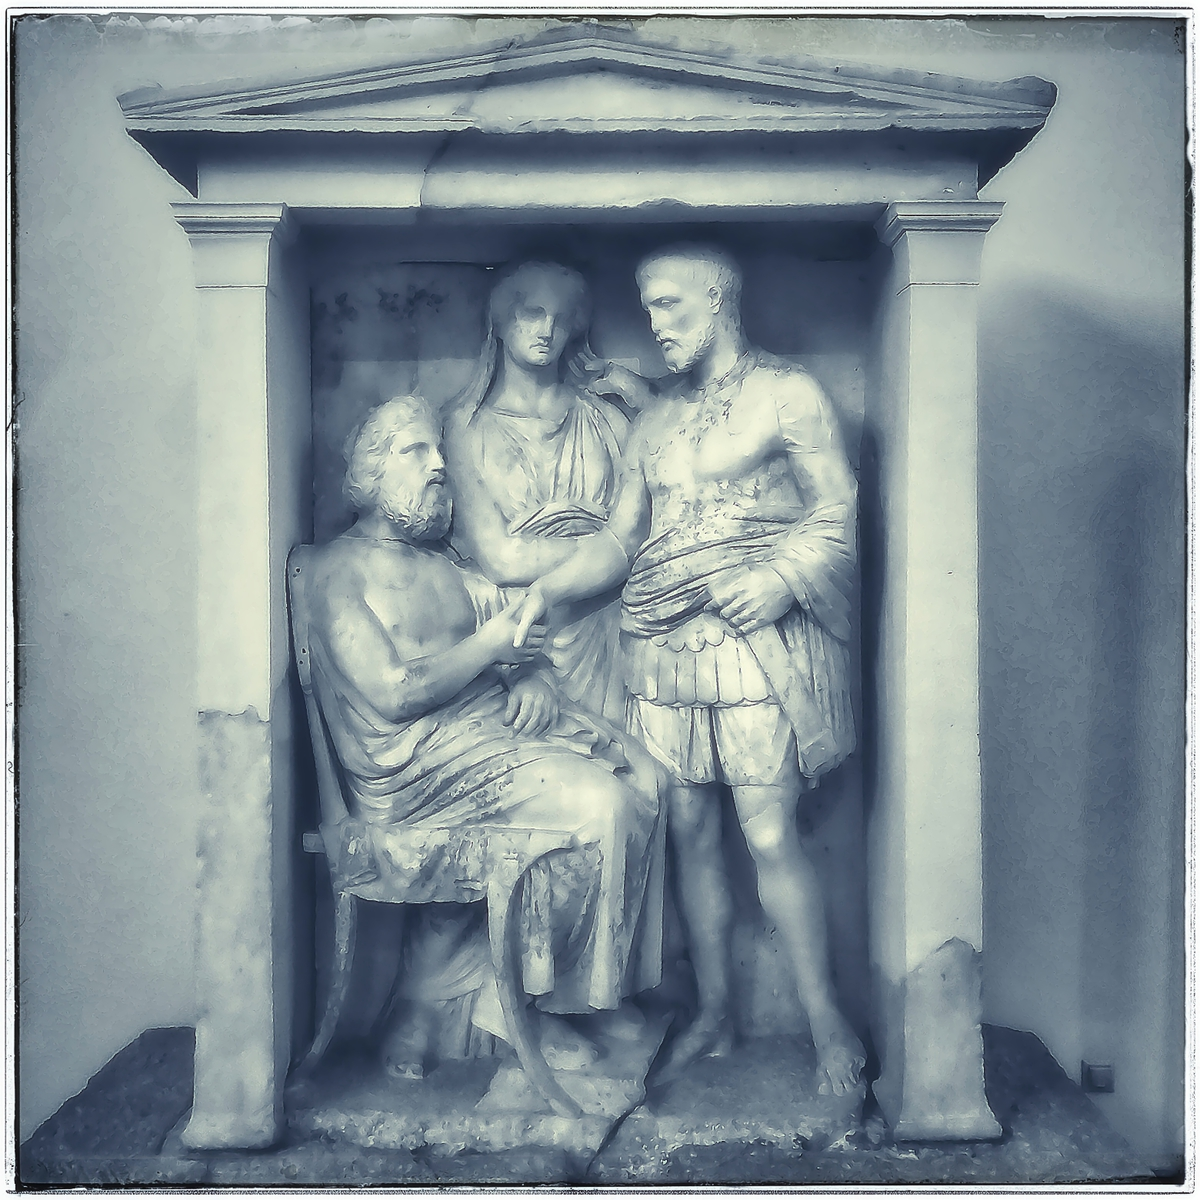
\includegraphics{thumb-lesson_V.jpeg}
  \caption{Museo Nazionale di Archeologia di Atene}
  \label{fig:textfig}
  %\zsavepos{pos:textfig}
  \setfloatalignment{b}
\end{figure}

\nobibliography{greekBiblio}
\bibliographystyle{alpha}


\end{document}
